
\chapter{Resultados Experimentais }
\label{cap:resultados}

\section{Resultados}


\subsection{RC3, RC7 e RC28}

Assim como feito em \cite{greciaLin}, iremos usar dados supostos disponíveis diariamente no chão de fábrica. Portanto, para um lote recém expedido,
não podemos usar os índices RC3 e RC7 para auxiliar na predição de RC28. Dessa maneira, iremos usar os últimos índices RC3 e RC7 disponível para o lote expedido no dia $t$,
i.e. o índice RC3 do dia $t-3$ e RC7 do dia $t-7$, que acabaram de ser medidos. \\


\subsection{Abordagem Não-Temporal}

 Para ambos as classes de modelos os dados foram transformados para possuirem variância
unitária e média 0. Os índices RC3 e RC7 foram usados como entrada e o índice
RC28 foi usado como saída. Os dados foram divididos em
\textit{treino}, \textit{validação}. Usamos os dados de treino 
para treinar os
modelos, e os de validação apenas para avaliar o seu erro. O Gráfico
~\ref{fig:divrc28} mostram essa divisão. Lembramos que apenas os dados de
validação são inéditos para os modelos, com eles avaliamos a capacidade de
generalização dos modelos. 


\begin{figure}[H]
  \centering
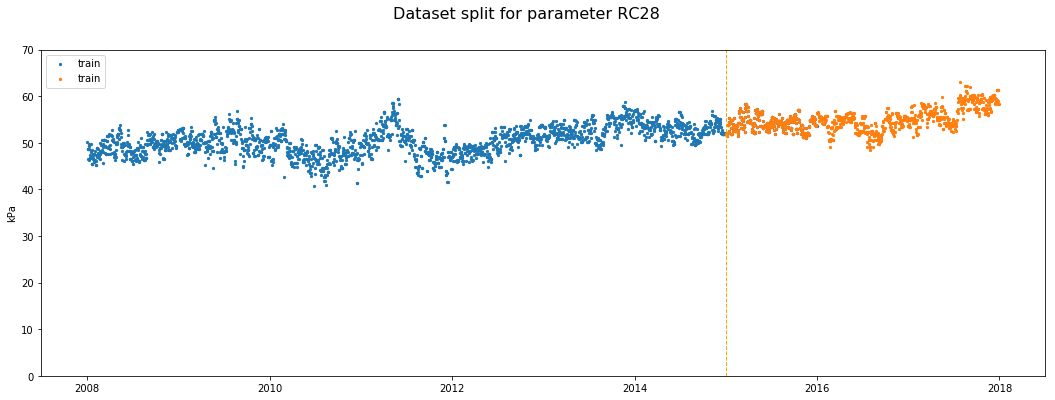
\includegraphics[width=0.9\columnwidth]{split_2008-2015-2017RC28.png}
\caption{Divisão do dataset para a saída RC28, os pontos azuis foram usados para
treino e os pontos laranjas usados para validação.}
  \label{fig:divrc28}
\end{figure}


\subsection{Modelos Bayesianos para Séries Temporais}


Todos os modelos foram implementados usando a bibliteca Pytorch \cite{pytorch}, para os Processos Gaussianos usamos a biblioteca GPyTorch \cite{gpytorch}. Para as predições de séries temporais, usamos todas as entradas de 01/2007 até 09/2018 como nossos dados de treino, e os últimos 3 meses de dados como os dados de validação. As tuplas de treino são da forma $(RC28_{t},\{\})$. Os dados são normalizados pelo método min-max para igualarmos suas grandezas. O vetor normalizado $z$ é dado pela seguinte equacão:  


\begin{equation}
z=\frac{x-\min (x)}{\max (x)-\min (x)}
\end{equation}


As Imagem \ref{fig:rmseday}, mostra o RMSE médio dos modelos por dia a medida que o horizonte de predição aumenta. A Tabela \ref{tab:rmse} mostra o mesmo resultado porém apenas para a predicão de 24h, 3d e 7d. \\



\begin{figure}[H]
\label{fig:rmseday}
\centering
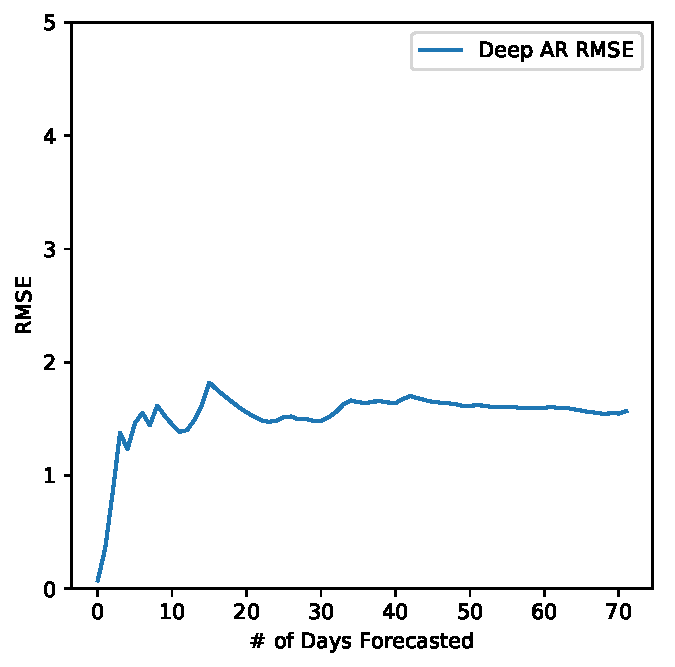
\includegraphics[width=.3\textwidth]{rmse_deep_ar.pdf} \hfill
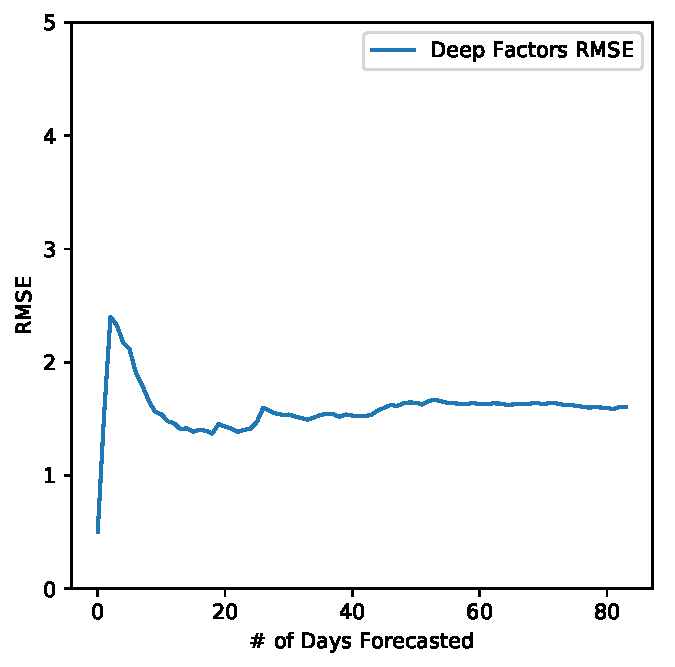
\includegraphics[width=.3\textwidth]{rmse_deep_factors.pdf} \hfill
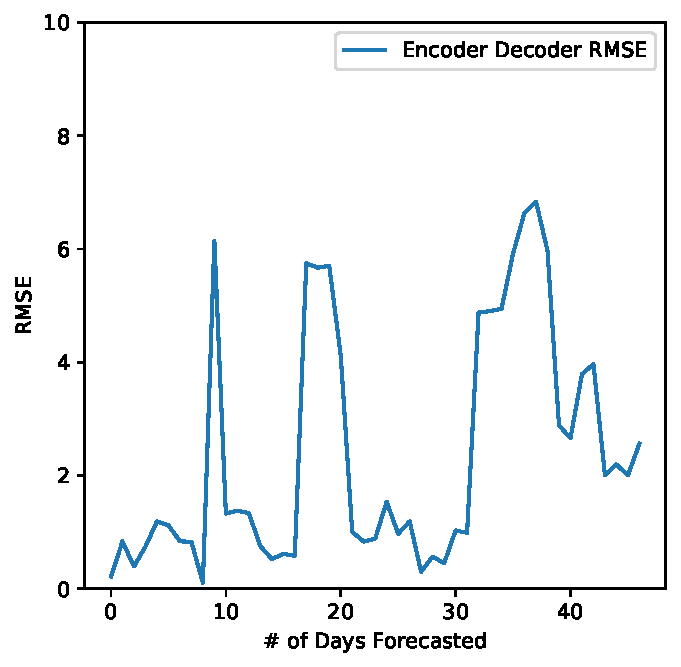
\includegraphics[width=.3\textwidth]{rmse_enc_dec.pdf} 
\caption{RMSE médio por dia para cada um dos modelos estudados} 
\end{figure}


\begin{center}
\begin{table}[htbp]
\caption{\label{tab:rmse}
RMSE values by forecast span}
\centering
\begin{tabular}{rr}
\hline
Deep Factors & RMSE\\
\hline
24h & 0.18\\
3d & 2.36\\
7d & 1.83\\
\hline
Deep AR & RMSE\\
\hline
24h & 0.07\\
3d & 1.37\\
7d & 1.44\\
\hline
Encoder Decoder & RMSE\\
\hline
24h & 0.22\\
3d & 0.36\\
7d & 1.04\\
\end{tabular}
\end{table}
\end{center}


Também estudamos a distribuição dos valores previstos, até 150 dias após a data onde começam os dados de validação, a Imagem \ref{fig:distr} permite comparar as distribuições previstas pelos 3 modelos:

\begin{figure}[H]
\label{fig:distr}
\centering
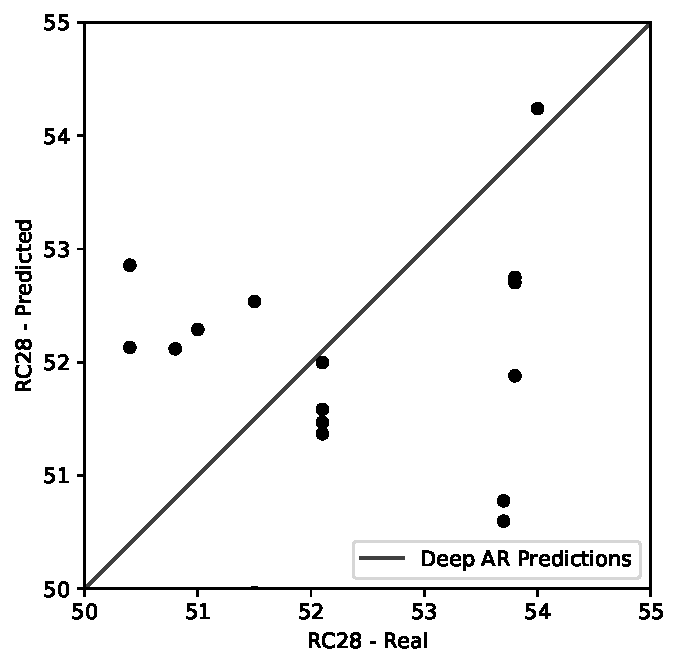
\includegraphics[width=.3\textwidth]{qq_deep_ar.pdf} \hfill
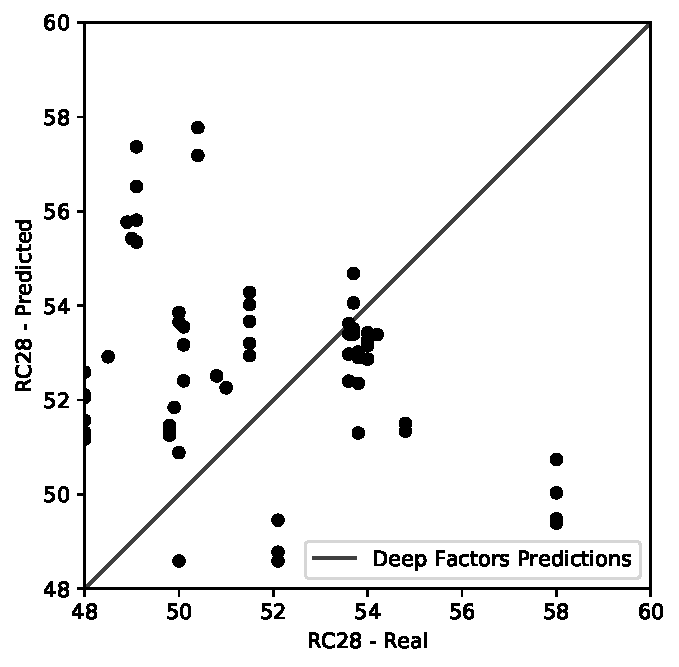
\includegraphics[width=.3\textwidth]{qq_deep_factors.pdf} \hfill
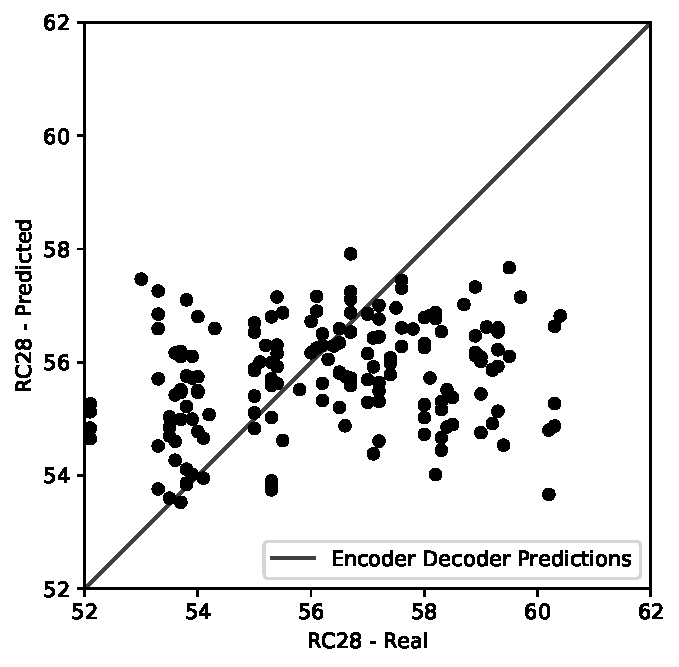
\includegraphics[width=.3\textwidth]{qq_enc_dec.pdf} 
\caption{Valores reais plotados contra os valores previstos para análise da distribuição aprendida por cada modelo} 
\end{figure}


Finalmente, os valores e incertezas previstos pelos modelos:


\begin{figure}[H]
  \label{fig:fordeepar}
  \centering
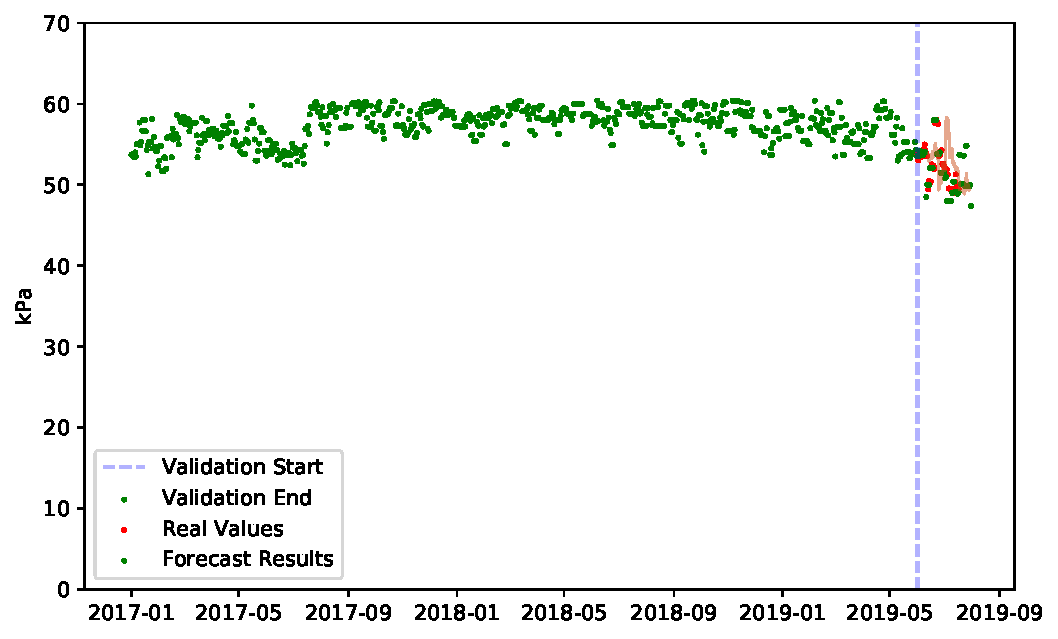
\includegraphics[height=.3\textwidth]{forecast_deep_ar.pdf} 
\caption{Predição para todos os dados de validação para o modelo Deep AR}
\end{figure}

\begin{figure}[H]
  \label{fig:fordeepfactors}
  \centering
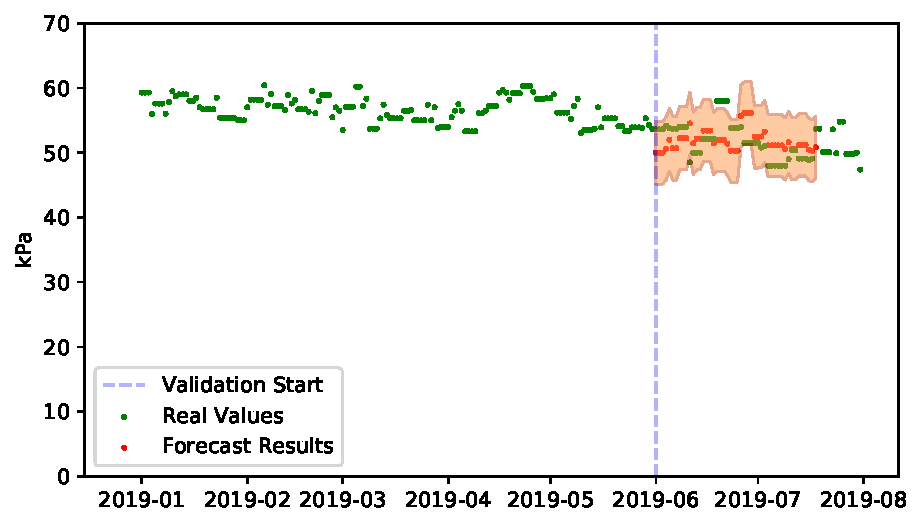
\includegraphics[height=.3\textwidth]{forecast_deep_factors.pdf} 
\caption{Predição para todos os dados de validação para o modelo Deep Factors}
\end{figure}

\begin{figure}[H]
  \label{fig:forencdec}
  \centering
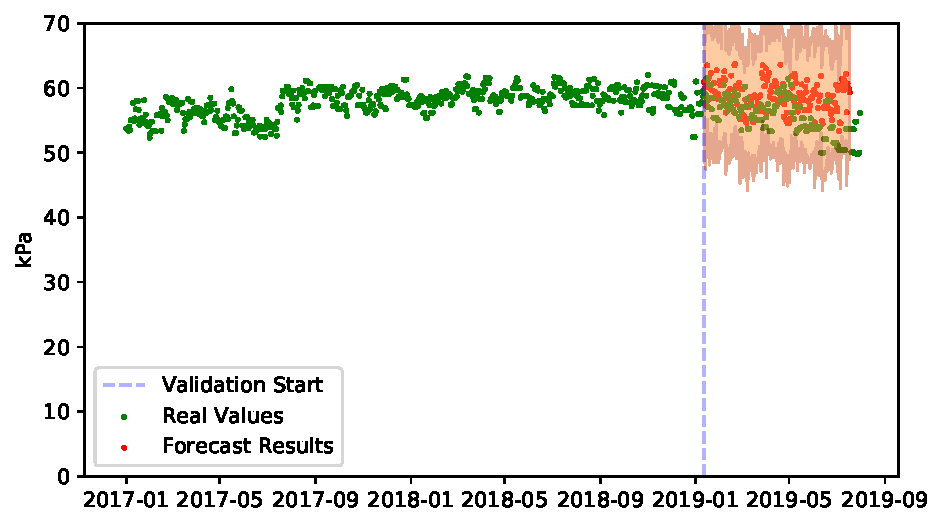
\includegraphics[height=.3\textwidth]{forecast_enc_dec.pdf} 
\caption{Predição para todos os dados de validação para o modelo Encoder Decoder Forecaster} 
\end{figure}
% Local Variables:
% TeX-master: "../quali"
% End:
